\documentclass[10pt]{scrartcl}
\usepackage[mdthm,colorsec,noauthor,noasy]{evan}
\usepackage{handout}
\usepackage[T1]{fontenc}
\usepackage{lmodern}
\usepackage{listings}
\lstset{language=Python,emptylines=1,basicstyle=\ttfamily\normalsize,identifierstyle=\color{black},keywordstyle=\color{NavyBlue},commentstyle=\color{black!60},stringstyle=\color{RawSienna},showstringspaces=false,columns=fullflexible,keepspaces=true,upquote=true,aboveskip=5pt,belowskip=5pt}
\newcommand{\py}[1]{\texttt{#1}}
\newcommand{\hint}[1]{\par\emph{Hint:} #1\par}
\newcommand{\codeblock}[1]{\par\noindent\begin{minipage}{\linewidth}\csname code#1\endcsname\end{minipage}\par}
\expandafter\def\csname codeswipe\endcsname{\lstinputlisting[firstline=4,lastline=10]{discussion_solutions.py}}
\expandafter\def\csname codeskip_fact\endcsname{\lstinputlisting[firstline=14,lastline=17]{discussion_solutions.py}}
\expandafter\def\csname coderecursive_prime\endcsname{\lstinputlisting[firstline=21,lastline=29]{discussion_solutions.py}}
\expandafter\def\csname codehailstone\endcsname{\lstinputlisting[firstline=33,lastline=45]{discussion_solutions.py}}
\expandafter\def\csname codesevens\endcsname{\lstinputlisting[firstline=49,lastline=68]{discussion_solutions.py}}
\expandafter\def\csname codekarel\endcsname{\lstinputlisting[firstline=72,lastline=84]{discussion_solutions.py}}
\expandafter\def\csname codeall_digits\endcsname{\lstinputlisting[firstline=4,lastline=9]{exam_solutions.py}}
\expandafter\def\csname codeprefix_process\endcsname{\lstinputlisting[firstline=13,lastline=21]{exam_solutions.py}}
\expandafter\def\csname codeprefix_loop\endcsname{\lstinputlisting[firstline=25,lastline=33]{exam_solutions.py}}
\expandafter\def\csname codenumbered_hailstone\endcsname{\lstinputlisting[firstline=37,lastline=47]{exam_solutions.py}}
\expandafter\def\csname codecollapse\endcsname{\lstinputlisting[firstline=51,lastline=58]{exam_solutions.py}}
\expandafter\def\csname codecontains\endcsname{\lstinputlisting[firstline=62,lastline=70]{exam_solutions.py}}
\expandafter\def\csname codereverse_curry\endcsname{\lstinputlisting[firstline=4,lastline=15]{examples.py}}
\expandafter\def\csname codeexp_parent\endcsname{\lstinputlisting[firstline=19,lastline=22]{examples.py}}
\expandafter\def\csname codesum_digits\endcsname{\lstinputlisting[firstline=26,lastline=30]{examples.py}}
\expandafter\def\csname codefact\endcsname{\lstinputlisting[firstline=34,lastline=37]{examples.py}}
\expandafter\def\csname codefact_iter\endcsname{\lstinputlisting[firstline=41,lastline=45]{examples.py}}
\expandafter\def\csname codefact_k\endcsname{\lstinputlisting[firstline=49,lastline=59]{examples.py}}
\expandafter\def\csname codeplay\endcsname{\lstinputlisting[firstline=63,lastline=72]{examples.py}}
\expandafter\def\csname codeparity\endcsname{\lstinputlisting[firstline=76,lastline=84]{examples.py}}
\expandafter\def\csname codecascade\endcsname{\lstinputlisting[firstline=88,lastline=92]{examples.py}}
\expandafter\def\csname codealice_bob\endcsname{\lstinputlisting[firstline=96,lastline=108]{examples.py}}
\expandafter\def\csname codeunique_factors\endcsname{\lstinputlisting[firstline=112,lastline=127]{examples.py}}
\expandafter\def\csname codefib\endcsname{\lstinputlisting[firstline=131,lastline=136]{examples.py}}
\expandafter\def\csname codepartitions\endcsname{\lstinputlisting[firstline=140,lastline=147]{examples.py}}
\expandafter\def\csname codeparking\endcsname{\lstinputlisting[firstline=151,lastline=156]{examples.py}}
\expandafter\def\csname codestreak\endcsname{\lstinputlisting[firstline=160,lastline=162]{examples.py}}
\expandafter\def\csname codenum_eights\endcsname{\lstinputlisting[firstline=4,lastline=9]{hw_solutions.py}}
\expandafter\def\csname codedistance\endcsname{\lstinputlisting[firstline=13,lastline=16]{hw_solutions.py}}
\expandafter\def\csname codeinterleaved\endcsname{\lstinputlisting[firstline=20,lastline=29]{hw_solutions.py}}
\expandafter\def\csname codecoins\endcsname{\lstinputlisting[firstline=33,lastline=49]{hw_solutions.py}}
\expandafter\def\csname codemax_subseq\endcsname{\lstinputlisting[firstline=53,lastline=58]{hw_solutions.py}}
\expandafter\def\csname codehanoi\endcsname{\lstinputlisting[firstline=62,lastline=73]{hw_solutions.py}}
\expandafter\def\csname codeanonymous\endcsname{\lstinputlisting[firstline=77,lastline=81]{hw_solutions.py}}

\title{CS 61A --- Week 4}
\subtitle{Solutions: Discussion 3, HW3 and assigned real exams}
\author{}\date{}\ihead{}
\begin{document}\maketitle
\section{Discussion 3 and related Lecture 10 practice}
\begin{prob}
\textbf{Q1: Swipe.} \idea{The first and last output lines are the current last digit. A smaller call produces exactly the lines between them.}
\codeblock{swipe}
\begin{steps}
\ii A one-digit input needs one line, so the supplied base prints it once. For a longer input, remove the last digit before recursing.
\ii For 2837 the calls first print 7,3,8,2. The call on 2 returns with no second print; the waiting calls then print 8,3,7. Each call returns None.
\ii Positive integer division by 10 eventually reaches one digit. The implementation uses no loops, string conversion or indexing.
\end{steps}
\end{prob}
\begin{prob}
\textbf{Q2: Skip Factorial.} \idea{Remove the first factor n; the remaining product is exactly the skip factorial of n-2.}
\codeblock{skip_fact}
\begin{steps}
\ii For positive n, the condition n $\le2$ covers both final possible factors 1 and 2. Return that factor directly.
\ii Otherwise multiply n by the smaller product. Thus 5 gives $5\cdot3\cdot1=15$, and 8 gives $8\cdot6\cdot4\cdot2=384$. Decreasing by 2 reaches the base in either parity.
\end{steps}
\end{prob}
\begin{prob}
\textbf{Q3: Is Prime.} \idea{The original n stays fixed; only the next candidate divisor changes. Retaining n in a parent frame makes one helper argument sufficient.}
\codeblock{recursive_prime}
\begin{steps}
\ii The helper's promised result is whether none of i through $n-1$ divides n. At i=n there are no candidates left, so return true; n itself is not tested as a disqualifying proper divisor.
\ii A divisor at i disproves primality and returns false. If i does not divide n, checking i+1 through $n-1$ is precisely the remaining task.
\ii With n $>1$, the initial candidate 2 is valid and each step decreases the candidates remaining. For 2 the base returns true;16 fails at 2;521 has no candidate divisor and returns true. An external helper would need n as another argument, since it would not have this retained parent binding.
\end{steps}
\end{prob}
\begin{prob}
\textbf{Q4: Recursive Hailstone.} \idea{Print the current term once, then ask the appropriate helper for this term plus the length of the rest.}
\codeblock{hailstone}
\begin{steps}
\ii At 1, hailstone prints 1 and calls odd, which returns 1. This is one element, not zero transitions.
\ii An even input continues to n//2; an odd input above 1 continues to 3n+1. A helper adds 1 to that returned term count to include the current printed term.
\ii For 10 the call arguments are 10,5,16,8,4,2,1 and the counts on return are 1,2,3,4,5,6,7 in reverse order. The first call returns 7. This proves the count whenever the sequence terminates; it does not prove all positive starts terminate.
\end{steps}
\end{prob}
\begin{prob}
\textbf{Q5: Sevens.} \idea{The current speaker has already been determined; a number divisible by 7 or containing 7 determines where the next turn goes.}
\codeblock{sevens}
\begin{steps}
\ii The helper invariant is: player who says i, and direction gives the movement order before applying i's rule. At i=n that is the requested answer, so return before another move.
\ii Otherwise reverse at a qualifying i, advance once in the resulting direction, wrap 1--k, and recurse on i+1. This preserves the state interpretation and reaches n after finitely many increments.
\ii For 5 players, the exact speakers for 1 through 20 are $1,2,3,4,5,1,2,1,5,4,3,2,1,5,1,2,3,2,1,5$. In particular the source's 2,6,7,8,9,18 cases give 2,1,2,1,5,2. At 7,14 and 17 the direction reverses after that number is said.
\end{steps}
\end{prob}
\begin{prob}
\textbf{Spring 2024 MT1 Q4(e): Streak.} \idea{A longer streak consists of a shorter valid streak whose last digit agrees with the one removed.}
\codeblock{streak}
\begin{steps}
\ii The first group accepts the one-digit bases 1--6. For a longer n, compare n\%10 with(n//10)\%10 and recursively check n//10. These fill the two source blanks.
\ii If the recursive prefix is a valid equal-digit dice integer and its last digit matches the removed one, every original digit is equal and valid. Removing digits eventually reaches the one-digit base; a repeated 9 eventually fails there.
\ii Thus 22222,4,33333333333333 pass.22322 fails at a digit change;99999 fails its final 9 base;505,707,7070 fail either digit agreement or the invalid one-digit base. All actual source examples are covered.
\end{steps}
\end{prob}
\begin{prob}
\textbf{Q6 (optional): Karel.} \idea{A smaller call advances through the remaining row and returns facing west; each waiting call then needs only one move back.}
\codeblock{karel}
\begin{steps}
\ii A call starts facing east with L squares left including its current square. If L=1, turn west and stop. If L=2, move to the last square, turn west and stop. These are the two base branches.
\ii For L $\ge3$, advance two squares and solve the same task on L $-2$ squares. By its contract, the smaller call finishes facing west at offset $\lfloor(L-2)/2\rfloor$ from its own start. One more move west gives offset $2+\lfloor(L-2)/2\rfloor-1=\lfloor L/2\rfloor$ from the original start.
\ii Thus the final column is $1+\lfloor n/2\rfloor$:4 for n = 7, and the right of the two middle columns for even n. Every forward move is guarded by a clear test. The return move is safe because its smaller call started at least two squares east of the waiting call.
\ii All branches end facing west. The function uses only conditionals and calls in its body, including its recursive call; it never reads or stores n. The linked UI starts bottom-left facing east; the proof uses that initial heading.
\end{steps}
\begin{fig}
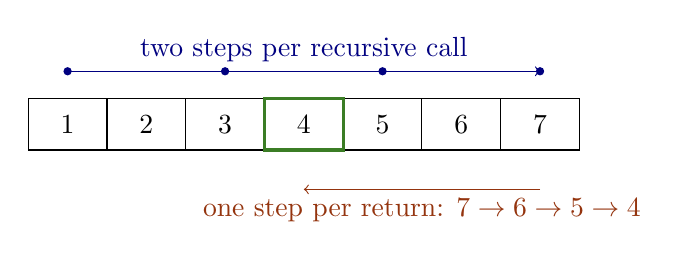
\begin{tikzpicture}
\foreach \i in {1,...,7}{\draw (\i,0) rectangle +(1,.65);\node at (\i+.5,.32) {\i};}
\draw[OliveGreen,very thick] (4,0) rectangle +(1,.65);
\draw[->,NavyBlue] (1.5,1)--node[above]{two steps per recursive call}(7.5,1);
\foreach \x in {1.5,3.5,5.5,7.5}{\fill[NavyBlue] (\x,1) circle (1.5pt);}
\draw[->,RawSienna] (7.5,-.5)--node[below]{one step per return: $7\to6\to5\to4$}(4.5,-.5);
\end{tikzpicture}
\figcap{For the actual 7-square example, the calls begin at columns 1,3,5,7. Turning west at the end and taking one return move per waiting call reaches column 4.}
\end{fig}
\end{prob}

\section{Homework 3}
\begin{prob}
\textbf{Q1: Num Eights.} \idea{Use the last digit to decide whether to add1 to the count on the shorter prefix. No variable assignment is needed.}
\codeblock{num_eights}
\begin{steps}
\ii A one-digit number contributes 1 precisely when it is 8. A longer number contributes the shorter prefix's count, plus 1 only when its last digit is 8.
\ii For 8782089, the successive tested digits are 9,8,0,2,8,7,8; three contribute 1. This gives 3. The source's remaining inputs 3,8,88888888,2638,86380,12345 give 0,1,8,1,2,0.
\ii Removing a digit reaches a one-digit base. The entire function contains no assignment or loop statement; its branches call the same recursive count.
\end{steps}
\end{prob}
\begin{prob}
\textbf{Q2: Digit Distance.} \idea{Removing the last digit removes exactly the final adjacent pair; all earlier pairs remain unchanged.}
\codeblock{distance}
\begin{steps}
\ii A single digit has no pair and contributes 0. Otherwise add the absolute difference between the last two digits to the distance of n//10.
\ii For 71253, the right-to-left pair contributions are 2,3,1,6, with sum 12. For 314 they are 3 and 2, with sum 5;777 gives 0. The longer source cases 31415926535 and 3464660003 give 32 and 16.
\ii Integer division removes one digit on each call; no pair is counted twice or omitted, and there are no loops.
\end{steps}
\end{prob}
\begin{prob}
\textbf{Q3: Interleaved Sum.} \idea{Alternate the function being called instead of testing an index's parity.}
\codeblock{interleaved}
\begin{steps}
\ii odd(k) is called only at odd k; it applies f\_odd there and asks even for k+1. The even helper does the corresponding even step and asks odd for the next index.
\ii Above n, no terms remain and the result is 0. Increasing k terminates, and the alternating calls include each index 1 through n once.
\ii With identity/square and n = 5, the sum is $1+4+3+16+5=29$. Reversing them gives $1+2+9+4+25=41$. At n = 4, triple/square gives $3+4+9+16=32$; square/triple gives $1+6+9+12=28$.
\ii The implementation uses addition and comparison only to advance/control indices. It contains none of the operators or loops banned by the public tests; supplied term functions may perform their own arithmetic.
\end{steps}
\end{prob}
\begin{prob}
\textbf{Q4: Count Coins.} \idea{At each denomination, separate combinations that use at least one such coin from combinations that use none.}
\codeblock{coins}
\begin{steps}
\ii The supplied next\_smaller\_coin returns 10,5,1 and then None. The helper's result counts combinations totaling remaining with the current coin and smaller denominations.
\ii Using a current coin leaves remaining $-$ coin and permits more copies of that coin. Using none leaves remaining unchanged and lowers the denomination. Those cases are disjoint and exhaustive, so add their counts.
\ii At remaining 0, the coins already selected complete one combination. Negative remaining is impossible; a positive remaining with coin None is impossible. The success test comes first, so completing a total counts even when no denominations remain.
\ii For 15, the six combinations are exactly those listed in the problem. The source totals 10,20,45,100,200 give 4,9,39,242,1463. Every recursive branch either lowers the positive remaining amount or advances along a finite denomination list; it terminates with no loops.
\end{steps}
\end{prob}
\begin{prob}
\textbf{Q5: Maximum Subsequence.} \idea{Every candidate either uses the current last digit or omits it. Find the best candidate in each group, then compare.}
\codeblock{max_subseq}
\begin{steps}
\ii If no digits or no slots remain, the best numeric result is 0. Otherwise keeping the last digit uses a slot and appends it to the best preceding result; skipping it leaves the slot limit unchanged.
\ii Multiplying by 10 and adding a fixed digit preserves numerical order. Therefore the best preceding subsequence also gives the best candidate that keeps this last digit. Taking the maximum covers both exhaustive groups.
\ii For $n=2012,t=2$, the keep-last branch gives $2\cdot10+2=22$ and the skip-last branch gives 21; return 22. For $n=20125,t=3$, keeping 5 gives 225 while skipping it gives 212.
\ii The source's other cases give 20125 at limits 5 or 6,345 at 12345/limit 3,0 at limit 0, and 5 at limit 1. Every call removes a digit; the implementation uses recursion and no loops.
\end{steps}
\end{prob}
\begin{prob}
\textbf{Q6 (just for fun): Towers of Hanoi.} \idea{The largest disk cannot move until the smaller stack is off it, and its destination must also be free of smaller disks. With three rods, the spare rod is forced.}
\codeblock{hanoi}
\begin{steps}
\ii One disk needs exactly the supplied print\_move. For n $>1$, move the top $n-1$ disks to the spare rod. The recursive contract preserves their legal order.
\ii The largest disk is now exposed and the destination has no smaller disk, so move it. Transfer the smaller stack from spare to destination using the same recursive contract; all disks are now in their required order.
\ii The three rod labels sum to 6, so the spare rod is 6 $-$ start $-$ end. Each recursive stack has fewer disks and eventually reaches one disk. Larger disks below these subproblems do not obstruct their smaller disks.
\ii For n = 2,start 1,end 3, the moves are 1 $\to$2,1 $\to$3,2 $\to$3. For n = 3 the exact source sequence is 1 $\to$3,1 $\to$2,3 $\to$2,1 $\to$3,2 $\to$1,2 $\to$3,1 $\to$3. Each is printed using the given wording.
\end{steps}
\begin{fig}
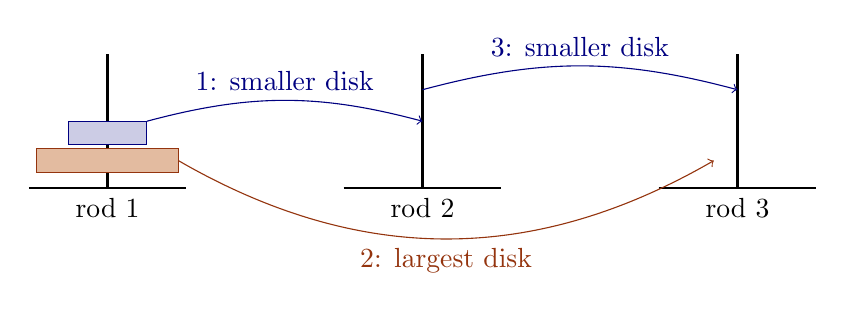
\begin{tikzpicture}
\foreach \x/\i in {0/1,4/2,8/3}{\draw[thick] (\x,-.2)--(\x,1.5);\draw[thick] (\x-1,-.2)--(\x+1,-.2);\node[below] at (\x,-.2) {rod \i};}
\draw[fill=RawSienna!25,draw=RawSienna] (-.9,0) rectangle (.9,.3);
\draw[fill=NavyBlue!20,draw=NavyBlue] (-.5,.35) rectangle (.5,.65);
\draw[->,NavyBlue] (.5,.65) to[bend left=15] node[above]{1: smaller disk}(4,.65);
\draw[->,NavyBlue] (4,1.05) to[bend left=15] node[above]{3: smaller disk}(8,1.05);
\draw[->,RawSienna] (.9,.15) to[bend right=30] node[below]{2: largest disk}(7.7,.15);
\end{tikzpicture}
\figcap{The actual 2-disk case: move the smaller disk aside before the largest can move, then place it back above the largest. For n disks, replace the smaller disk by the ordered top n-1 stack.}
\end{fig}
\end{prob}
\begin{prob}
\textbf{Q7 (just for fun): Anonymous Factorial.} \idea{A function parameter can supply the self-reference that a global def-name would usually supply.}
\codeblock{anonymous}
\begin{steps}
\ii The first lambda receives a function f and returns a function of n calling f(f,n). The argument supplied for f is the second lambda, which accepts its own function value as its first parameter.
\ii Its recursive branch uses f(f,$n-1$), passing that same value again. Thus every recursive application has access to itself without a global recursive name. At 0 it returns 1; at positive n it multiplies n by the result at $n-1$.
\ii The resulting function at 5 returns 120. Its return expression uses only lambdas, calls and a conditional expression, with no reference to make\_anonymous\_factorial. The imports precede their use. The original source's named lambda example instead refers to global fact; this expression removes that dependency.
\end{steps}
\end{prob}

\section{Assigned real exams}
\begin{prob}
\textbf{Fall 2017 MT1 Q4(a): Collapse.} \idea{If the last two digits agree, discard the last copy; otherwise preserve the last digit after collapsing the earlier digits.}
\codeblock{collapse}
\begin{steps}
\ii left = 0 means n has one digit, including n = 0; return last. Otherwise left's last digit is the digit immediately to last's left.
\ii If these agree, removing the current last digit leaves one fewer copy of the same consecutive run. If they differ, the collapsed prefix ends in left's last digit and can safely have last appended without creating a duplicate boundary.
\ii For 12234441, collapsing each run gives 1,2,3,4,1 and result 12341. For 11200000013333 it gives 1,2,0,1,3 and 12013. Inputs 1234,0,3 remain unchanged. Each call strips a digit and preserves all nonduplicate transitions.
\end{steps}
\end{prob}
\begin{prob}
\textbf{Fall 2019 Final Q6(b): Contains.} \idea{For the requested last digit, choose the rightmost matching digit available in b. This leaves as much of b's prefix as possible for all earlier requested digits.}
\codeblock{contains}
\begin{steps}
\ii Equal a,b succeeds immediately. A decimal subsequence cannot have a greater numeric value than its source: using fewer digits gives a shorter value, while using all digits leaves the same number. Thus a $>$ b fails.
\ii If last digits agree, match them and remove both. Any successful placement of a's last digit could be shifted right to this last position, leaving all its earlier matches available. This justifies choosing the matching last digit without another branch.
\ii If last digits differ, b's last digit cannot match the last requested digit and must be discarded. Keep a while shortening b. Every call shortens b until success or failure is decided.
\ii For 357 in 12345678, skip 8, match 7, skip 6, match 5, skip 4, match 3, then no requested digits remain: true. For 753 the requested order fails;357 in 37 lacks 5 and fails.
\ii The official convention represents an empty remainder by a = 0, even on initial input. Hence contains(0,7) is true under that convention, not a claim that the ordinary one-digit numeral 0 occurs in 7. The implementation uses none of the forbidden conversions, containers or indexing syntax.
\end{steps}
\end{prob}

\end{document}
